\documentclass[a4paper, 12pt]{article}

\usepackage{graphicx}
\usepackage{amsmath}
\usepackage{amsfonts}
\renewcommand{\figurename}{Fig.}
\usepackage[labelsep=period]{caption}
\usepackage{subfigure}% in preamble
\usepackage{secdot}
\usepackage{titlesec}
\usepackage{lineno}
\usepackage{helvet}
\usepackage{rotating}
\usepackage{tabularx}


\renewcommand{\familydefault}{\sfdefault}
\topmargin -.5 in \oddsidemargin .5 in \textwidth 5.75 in \textheight 9in
%\linenumbers

\titleformat{\subsection}
  {\normalfont\large\itshape}{\thesubsection}{3em}{}


\date{}
\title{{\bf Long-Range Violent Typhoon Forecasting: A Machine-Learning Approach}}
\vspace{.2in}
\author{{\bf Paul ISIHARA}\footnote{ Corresponding author:  Paul Isihara, Department of Mathematics, Wheaton College, Wheaton IL 60187 USA. email:paul.isihara@wheaton.edu}, {\bf Jacob CLEMENT}, {\bf Korey CLEMENT},{\bf Daniela CUBA}, \\{\bf Danilo R. DIEDRICHS},  {\bf Peyton FINLEY},   {\bf Michaela FLITSCH}, {\bf Roland HESSE}, \\ {\bf Spencer HILLS},   {\bf Michael KIETZMAN},  {\bf Kyu Lim LEE}, {\bf Mark NUSSBAUM}.\\{\bf Zach OSLUND},   {\bf Kaile  PHELPS},
 {\bf Jenny RUDA}, {\bf Matthew RUEGER}, \\{\bf Erica SWAIN},  {\bf Kei TAKAZAWA},  and {\bf Emily WILLSON}\\\vspace{.5in}\emph{Department of Mathematics, Wheaton College, IL USA}}
\date{December 18, 2018}



\begin{document}
\pagenumbering{gobble}
\maketitle


\linespread{2}

\newpage
\pagenumbering{arabic}
\normalsize

\abstract{

The  enormous devastation caused by typhoon Haiyan (2013)  led us to consider recent Japan Meteorological Agency (JMA) violent typhoons (sustained wind speeds of at least 105 knots) as a special category of research. Using JMA best-track data for the years 2009-2013 as training data, we construct a quasi-operational MATLAB machine learning model which uses best track data for the first 24 hours of an emerging tropical storm as predictors, and has the storm category, as well as a latitude, longitude, and maximum sustained wind speed as responses. The model is tested using 2014-2016 best track data, for which the quasi-operational Prediction error is reported as a confusion matrix for the category of the storm. and in comparison with a baseline climatological regression model for violent typhoon position and maximum wind speed. 




{\flushleft {\bf Keywords} JMA best track, MATLAB machine learning model, confusion matrix, regression model}
\newpage


\section{Introduction}

The  enormous devastation caused by typhoon Haiyan (2013) led us to consider quasi-operational prediction (``hindcasting'') of JMA Grade 5 violent typhoons (maximum sustained wind speeds of at least 105 knots or 194 km/hr)  as a special category of research.   As has been the case for decades (Epstein 1969; Hope and Neumann 1970; Leith 1974; Anthes 1982;  Krishnamurti et al. 1991; Wu and Emmanuel 1993; Elsberry 1995 and Leslie et al. 1998),  in recent years, understanding of physical processes (Chan, 2005; Cap 2006; Rozanova et al. 2010; Yanase et al. 2010 and  Yang et al. 2012) combined with advanced numerical, statistical ensemble and other data assimilation methods  (Krishnamurti et al. 1999; Williford et al. 2003;  Weber 2005; Meng et al. 2007;  Chan 2010;  Cecelski et al. 2014; Chang et al. 2014 and Higaki et al. 2015) have resulted in steady improvement of operational typhoon forecasting  (Korean Meteorological Administration 2013 and Japan Meteorological Agency 2015).  At the same time, sensitive dependence on initial conditions (Lorentz 1963, 1965; Kamaromi et al. 2011; Yamaguchi et al. 2012 and Chang et al. 2014) and `busted cases'  with large track position errors (Ito and Wu 2013), have kept the door open for new approaches to improve both operational and no-skill baseline long range typhoon forecasting models. In this study, a MATLAB machine learning model (MMLM) built from best track data for the first 24 hours of a tropical storm as predictor variables, and the category of the storm, as well as location and maximum wind speed as responses,  


  In developing a new model for this special category of research, we considered only  best track data for the years 2009-2016  published by the Japan Meteorological Agency (JMA 2009-2016) which is downloadable at  http://www.jma.go.jp/ jma/jma-eng/ jma-center/ rsmc-hp-pub-eg/trackarchives.html. Data for the years 2009-2013 were used to train the model, and 2014-2016 to test the model. A confusion matrix is used to analyze error in quasi-operational storm category predictions.  For the position and maximum wind speed, we considered only the violent typhoon category for which the MML model response was compared to a multiple linear regression (MLR) model developed in an earlier stage of this project.
  
  
  

   In Section 3 we describe an MLR model for long-range violent typhoon predictions. We identify each violent typhoon by a three coordinate \emph{genesis point} (GP) (latitude, longitude, pressure) giving the respective JMA best track point latitude, longitude and central pressure values at time $t=0$. We require a genesis point to have a recorded best track wind speed of 0 since wind speed is not one of the GP coordinates. The best track of each violent typhoon must have at least one \emph{violent point} whose coordinates (time, latitude, longitude, pressure, wind speed) are the respective time (in hours), latitude, longitude, central pressure (in hPa) and sustained maximum wind speed (in knots) best track values at any time point when the storm's maximum wind speed is at least 105 knots. A \emph{most violent point} (MVP) of a storm is defined to be any violent point with highest sustained maximum wind speed among the storm's violent points. Our goal was to create a simple `GP/MVP' multiple linear regression model, meaning one which uses just a storm's GP to predict an MVP under the assumption that the storm becomes violent.
   
   A default GP/MVP model is introduced, one which uses data for the seven violent typhoons between 2009-2012 to `hindcast'  MVPs of the 5 violent typhoons in 2013. To check robustness of the default GP/MVP model, 2010-2013 data was used to predict MVPs of the 4 violent typhoons in 2014.   In Section 3, we explain how an annual average predicted MVP track position error (EGP) compared favorably with a related JMA PER model error EP. In Section 4, strategies are introduced to reduce EGP by filtering the data used in regression. Monte Carlo simulation is used to assess the likelihood the EGP error was achievable by chance rather than information contained in past violent typhoon data.

    Multiple regression based typhoon models are of course far from new. They were introduced over 50 years ago (Arakawa 1964) and later employed in  both climatology persistence (CLIPER) and statistical typhoon intensity prediction (STIPS) models (Neumann 1972; Knaff et al. 2005 and Jin 2008). The real-time availability of global weather data together with super computer execution of physics-based models used in  current operational typhoon prediction has in general relegated statistically-based position forecasts using past climatological records to `no-skill' baseline predictions.  Position errors in climatological models serve as a baseline for prediction accuracy and an indicator of the relative difficulty in forecasting a particular storm. Improvement of the baseline `no-skill' forecast motivates improvement in operational forecasting. The GP/MVP model uses only initial ($t=0$) latitude, longitude and pressure as predictor variables and so is simpler than the National Hurricane Center's (2009) CLIPER5 model, another multiple regression based climatology model for predicting typhoon position first developed in 1972 and extended in 1998 to provide forecasts out to 120 h (5 days). CLIPER5 uses more input variables than GP/MVP.  In addition to initial intensity, variables including latitude, longitude, date, and movement in the past 12 and 24 hours are based on evolving rather than solely genesis point data. CLIPER5 is also used to predict entire storms of any intensity  rather than just MVPs of violent typhoons. Whereas CLIPER5 is used as a baseline to evaluate the skill of an operational forecast, the GP/MVP model offers a new early warning data point not currently provided by operational forecasting.

    Since the GP/MVP model uses only initial data (time $t=0$), it offers a different type of prediction than the physics based operational models which depend on continuous updates to evolving local and global weather conditions.  Moreover,  GP/MVP forecasting requires only extremely small violent typhoon data sets and the simplicity of the default linear regression model makes  GP/MVP forecasting easily adoptable as a new information point in early-warning operational typhoon forecasting.



\subsection{The Default GP/MVP Model}

We begin by considering the color-coded 3 dimensional data visualization of 2009-2012 JMA grade 5 typhoon best track data shown in Figure 1. Best track latitude, longitude and pressure (in hPa) are used for the geometric coordinates, and maximum sustained wind speed (in knots) is represented by color.  The JMA best tracks begin at $t=0$ at which time the wind speed is usually recorded as 0. We call these points \emph{genesis points} (GPs) and they appear in dark blue.  Since the terminal best track points also have wind speeds recorded as 0, the dark blue points form two clusters, with genesis points in the right cluster and terminal points clustered towards the left. Points in between the genesis point and terminal point are separated by 6 hour time intervals. Since pressures are highest at the beginning and end of the best track, all the dark blue points appear in the top layer of the scatter plot's ``funnel".  The light green and yellow layers in the funnel correspond to typhoons (63-84 knots), the orange layer to very strong typhoons (85-104 kts), and the red layer to violent typhoons ($\ge$105 kts). Violent points (wind speeds at least 105 kts) appear in the red layer at the bottom of the funnel. Figure 2 gives a 2 dimensional representation of these violent points. Note in particular the confinement of violent points to a relatively small geographic region.

  \marginpar{\fbox{Fig. 1}}
  \marginpar{\fbox{Fig. 2}}


A special type of violent point called a most violent point (MVP) is a point(s) in a typhoon's best track which has highest maximum wind speed among the violent points. A violent typhoon may have multiple MVPs as shown in Table 1 which specifies the genesis, violent, and most violent points of the 7 violent typhoons in the years 2009-2012. For the purpose of using just a storm's genesis point (GP)  data to predict a most violent point (MVP) by means of multiple regression, the fact that the funnel narrows from the top layer towards the bottom layer in Figure 1, and similarly, the confinement of violent points in Figure 2, is important to achieving reasonable position accuracy.


   We consider a multiple linear regression model in which the genesis point latitude ($x_1$), longitude ($x_2$) and pressure ($x_3$) coordinates serve as the predictor variables and the dependent variables are the five coordinates of an MVP, namely time ($y_1$), latitude($y_2$), longitude ($y_3$),  pressure ($y_4$), and wind speed ($y_5$). Regression coefficients using the violent typhoon data in Table 1 are shown in Table 2A.
\marginpar{\fbox{Table 1}}

             Denote the 2009-2012 violent typhoon data regression coefficients for latitude $\alpha=(\alpha_0, \alpha_1, \alpha_2, \alpha_3)=(-708.14,-.254,.167,.699)$  and the regression coefficients for longitude $\beta=(\beta_0, \beta_1, \beta_2, \beta_3)= (-1827.084, -.799,$ $1.033, 1.807)$.  Given only the genesis point (lat$_0$,lon$_0$,pressure$_0$) of a violent typhoon in 2013, the default regression model hindcasts the  latitude and longitude of an MVP as
              \begin{eqnarray*}
       \textup{Predicted MVP latitude} & = & \alpha_0+ \alpha_1 \textup{lat}_0 +  \alpha_2 \textup{lon}_0 + \alpha_3 \textup{pressure}_0,\\
        \textup{Predicted MVP longitude} & = & \beta_0+ \beta_1 \textup{lat}_0 +  \beta_2 \textup{lon}_0 + \beta_3 \textup{pressure}_0.\\
       \end{eqnarray*}


\marginpar{\fbox{Table 2}}


         {\flushleft  In} a similar way, the time, maximum sustained wind speed and central pressure of an MVP can be predicted from just the genesis point for a total of $4 \cdot 5 = 20$ regression coefficients.  For example, for Utor, the genesis point is given by
         \begin{quote}
         \centering
         (lat$_0$,lon$_0$,pressure$_0$)=(12.1,136.6,1008),
         \end{quote}
         {\flushleft and}  the default regression model predicted MVP is

               \begin{quote}
                 \centering
          (time,lat,lon,pressure,wind speed)=\\(130.3(h),16.6$^o$,126.1$^o$,898.9(hPa),114.9(kts)).
          \end{quote}

{\flushleft We} call this method of predicting a storm's MVP from its GP the \emph{(default) GP/MVP model}.


\subsection{MLR Error Analysis}

         In constructing and improving the default GP/MVP model, we focus on the position error of the predicted MVP. To this end, we used the mathematical concept of distance between a point $P$ and a finite set of points $S$, namely, the minimum distance between $P$ and the points in $S$ (Figure \ref{fig2}). We define the position error in predicted MVP as the distance between the point  $P$=(Predicted MVP latitude,Predicted MVP longitude) and the set $S$ of actual MVPs for the storm being predicted. Table 3 gives these prediction errors for 2013 MVPs.


\marginpar{\fbox{Figure 3}}
 \marginpar{\fbox{Table 3}}


         Minimization of the average predicted MVP position error EGP for violent storms in a given year guided development of the GP/MVP model.  EGP was compared to JMA's EP (corresponding JMA no-skill PER model baseline error) and EO (average operational forecast position error) for the day closest to the time coordinate of the MVP used in computing the position error. For example, if the time of the actual MVP was 78 hours, we used the EO and EP 72-h (3 day) average position forecast error as comparisons. The default model EGP error of 835.6 km for 2013 was deemed reasonable since it fell between the EO average error of 314.6 km and the EP average error of 850 km.

          To check model robustness, we compiled 2010-2013 violent typhoon data for the regression, and analyzed the
           2014 MVP predictions.  The violent typhoon Genevieve was excluded from analysis since a genesis point was not given (a positive wind speed was reported at $t=0$).  The 2014 EGP error of 680.75 km again fell between the average EO error of 384.75 km and the average EP error of 1332.15 km (Table 3).

     Though our focus was on minimization of position error, Table 3 also reports the average wind speed error and error in predicted timepoint of an MVP. We simply note here that these errors were quite reasonable for both 2013 and 2014.

     Insight into the size of the 2013 EGP error is given by Monte Carlo simulation.  We use random numbers to create data used in regression (DUIR) having the same structure as the DUIR based on 2009-2012 violent typhoons (see Figure 4).  In particular, we choose 7 points at random (uniform distribution) from the rectangle bounding 2009-2012 violent typhoon GPs.  For each of these randomized GPs, we create an appropriate number of MVPs.  For example, for the 1st randomized storm we create 6 randomized MVPs, for the 2nd storm, 3 randomized MVPs and so on.     \marginpar{\fbox{Figure 4}} We then used the randomized data set to predict 2013 MVPs and computed the average predicted MVP error. A histogram (see Figure 5) constructed using 1,000 randomized trials show that a predicted average 2013 MVP position error of 821.1 km or less could have been achieved by a randomized data structure with empirical probability of roughly {\bf p}=.155.


        In what follows, we use Monte Carlo simulation to obtain such ${\bf p}$-values to assess strategies which reduce EGP errors. For example, the default GP/MVP model's 2014 EGP error of 680.75 km has a {\bf p} value of .571 (see Table 3B) and the 2015 EGP error of 583 km has a {\bf p} value less than .001.  Note that the heavily right-skewed histogram suggests possible occurrence of  ``busted cases" which greatly increase the value of EGP due to the small number of violent typhoons occurring in any given year.

  \marginpar{\fbox{Figure 5}}


\subsection{Distance Filtering of the Data used in Regression}
As stated earlier, our primary goal in genesis point prediction of MVPs is the minimization of the average predicted MVP geographic position error for violent typhoons occurring in a given year (EGP). Improving the accuracy of predicted wind speed and the time at which an MVP occurs are also important, but were not considered in this study.  One approach to reducing EGP is to filter the data used in regression (DUIR).  Several filtering strategies are possible.

     An intuitive strategy is to rank the violent storms in the DUIR by geographic proximity of their genesis points to the genesis point of the typhoon being predicted. Table 4 shows the result of filtering the DUIR of 2009-12 violent typhoons and using data from just the 3 storms with closest geographic proximity. This filtering is such that if the genesis point of a storm `X' in the DUIR is too far from the genesis point of the storm being predicted, all MVPs of X are deleted from the DUIR. This approach gave a 2013 EGP error of 608.6 km ({\bf p} =.008).  However, since the 2014 predictions using the 3 closest typhoons had an EGP of 1007.2 ({\bf p}=.886 ) this method was deemed unreliable.  One reason is that the number of MVPs is not the same for each violent typhoon; hence fixing the number of violent storms involves variability in the size of the DUIR. Furthermore, the distances to the 3 closest storms in the DUIR may also be quite different from one predicted storm to another.

 \marginpar{\fbox{Table 4}}

A second type of filtering takes into consideration pressure differences between genesis points in addition to the geographic separation. Given two genesis points $U=(u_1,u_2,u_3)$ and $V=(v_1,v_2,v_3)$ there are various possibilities for measuring the ``distance" $d(U,V)$ between $U$ and $V$.  One distance measure  found to be helpful in various applications  is a (weighted) $p$-norm ( $\ddot{\textup{U}}$ster, H. and R.F. Love, 2001) defined by

\begin{displaymath}
d(U,V)=[\Omega_1( \frac{u_1-v_1}{\sigma_{lat}})^p+\Omega_2(\frac{u_2-v_2}{\sigma_{lon}})^p+\Omega_3(\frac{u_3-v_3}{\sigma_{pres}})^p]^{1/p}.
\end{displaymath}


{\flushleft Standard} deviations of the latitude, longitude and pressure (respectively denoted $\sigma_{lat},$ $\sigma_{lon},$ and  $\sigma_{pressure}$) for the data used in regression  (DUIR)  are used to standardize differences, accounting for the differences in scale of the coordinate axes.  Note that when $p=2$, if the (non-negative) parameters $\Omega_1, \Omega_2$, and $\Omega_3$ called ``weights" are all set equal to one, ($\Omega_1=\Omega_2=\Omega_3=1$), the distance $d(U,V)$ becomes the usual Euclidean norm for the normalized data. If the value of $p$ is changed to $p=1$, the so called ``taxi-cab" metric is obtained where one is constrained to move parallel to a coordinate axis in measuring the (normalized) distance from $U$ to $V$.  Although pressure is not a geographic coordinate, Figure 1 suggests that a Euclidean or taxi-cab norm might be appropriate for measuring the distance between two genesis points.    Similar to the previous section which used geographic distance to rank violent storms in the data used in regression (DUIR),  one can use a $p$-norm (or other measure of distance) to filter the DUIR in an attempt to reduce the EGP error according to the algorithm shown in Table 5. Note that the data used in regression (DUIR) includes only storms whose genesis points are within a specified distance $r$ to the genesis point of the storm being predicted. If $r$ is sufficiently large, distances are immaterial and the model reverts to the default model.

   \marginpar{\fbox{Table 5}}


 In Table 6, we compare the default model EGP errors for 2013 - 2015 with those filtering the DUIR via the taxicab and Euclidean norms. In some cases, a particular norm can greatly reduce the default model error (eg. 2013 taxi-cab metric with $r=3$ has an EGP error of 537.9 ({\bf p} $<.01$)). However, the errors for both these $p$-norms fluctuate dramatically from year to year. The default model was more stable over the years tested (2013-2015).

\marginpar{\fbox{Table 6}}



Varying the weights allows one to place different amounts of importance on differences between coordinates.  For example, if a latitude difference in genesis points is deemed more important than either longitude or pressure difference, one would increase the value of $\Omega_1$ in relation to the weights $\Omega_2$ and $\Omega_3$.   Note that one can use a different $p$ norm measure for each of the 5 predicted MVP variables (time, lat, lon, pressure, wind speed). Since each distance measure has 4 parameters ($\Omega_1,\Omega_2,\Omega_3$ and $p$), and the radius $r$ is a 5$^{th}$ parameter specifying how close GPs must be for inclusion in the DUIR, there are a total of $5 \cdot 5 = 25$ $p$-norm model parameters that can be tuned in an attempt to improve MVP predictions. Finding the best distance measure for filtering the data used in regression is a difficult problem open to further investigation.




\section{MML model Error Analysis}

\subsection{Confusion Matrix for Storm Category Prediction Error}

\subsection{MVP Prediction Error}

\section{Summary and Conclusions}

Genesis point prediction of most violent points has humanitarian value in that such predictions seek to give the earliest advance warning of the most violent track points during a typhoon season. In GP/MVP models, real-time meteorological data, advanced algorithms embodying physical laws and statistical methods, and super computing power employed in operational forecasting are not utilized since only track position and central pressure at time $t$=0 can be used in the MVP forecast.  For 2013 and 2014, a default GP/MVP model has an average predicted MVP position error EGP which is between the JMA operational error (ER) and baseline PER model error (EP).
  The default model also performed well in 2015 when assessed by a Monte Carlo simulation (2015 JMA EP and EO errors were not published as of the writing of this article.)  As such, the default model GP prediction of an MVP could be included within current operational forecasting as shortly after $t=0$ as a point of information alerting people living near the predicted MVP to the greatest possible typhoon threat. In cases where the storm does not become violent and loses strength, MVP warnings are canceled to the relief of all concerned.  Further model refinement, including determination of effective $p$-norm or other filtering methods to improve the accuracy not only of predicted geographic position of MVPs, but also the time and wind speed at which these MVPs occur, is therefore deemed to be an important open research topic.

\newpage


\center{{\bf \large Acknowledgements}}


 The authors would like to thank Wheaton College's Summer Research  program and Alumni Association for their support of this project.

\center{{\bf \large References}}


\begin{list}{}{\leftmargin=1em \itemindent=-2em}


\item Anthes, R.A., 1982: \emph{Tropical cyclones. Their evolution, structure and effects.} American Meteorological Society.208 pp.

\item  Arakawa, H., 1964: Statistical method to forecast the movement and the central pressure of typhoons in the western north Pacific.  \emph{J. Appl. Meteorol.} {\bf 3}, 524-528.


\item Cap, F. 2006: {\em Tsunamis and Hurricanes: A Mathematical Approach.} Springer-Verlag, 201 pp.

\item Cecelski, S.F., D.-L. Zhang and T. Miyoshi, 2014: Genesis of hurricane Julia (2010) within an African easterly wave: developing and non-developing members from ERF-LETKF ensemble forecasts. \emph{J. Atmos. Sci.}, {\bf 71}, 2763-2781.

\item Chan, J.C.L., 2005: The physics of tropical cyclone motion. \emph{Annu. Rev. Fluid Mech.} {\bf 37}, 99-128.

\item Chan, J.C.L., 2010: Movement of Tropical Cyclones. \emph{Global Perspectives on Tropical Cyclones: From Science to Mitigation}, J.C.L. Chan and J.D. Keperts, eds., World Scientific Publishing, 133-148.


\item  Chang, C.-C., S.-C. Yang and C. Keppenne, 2014: Applications of the mean recentering scheme to improve typhoon track prediction:  a case study of typhoon Nanmadol (2011). \emph{J. Meteor. Soc. Japan} {\bf 92}, 559-584.



\item Elsberry, R., 1995: Tropical cyclone motion. \emph{Global Perspectives on Tropical Cyclones}, J.C. L. Chan and J.D. Kepert, Eds., World Meteorological Organization, 106-197.

\item Epstein, E.S., 1969: Stochastic dynamics prediction. \emph{Tellus}, {\bf 21}, 739-759.


\item Higaki, M., M. Kyouda and H. Yamaguchi, 2015: Upgrade of JMA's Typhoon Ensemble Prediction System. http://www.wcrp-climate.org/WGNE/Blue Book/2014/individual-articles/06\_Higaki\_Masakazu\_WGNE\_BB2014\_TEPS upgrade\_higaki.pdf


\item Hope, J. R. and C.J. Neumann, 1970: An operational technique for relating the movements of existing tropical cyclones to past tracks. \emph{Mon. Weather Rev.}, {\bf 98}, 925-933.


    \item Ito, K. and C. Wu, 2013: Typhoon-position-oriented sensitivity analysis. part I: theory and verification. \emph{J. Atmos. Sci.}, {\bf 70}, 2525-2546.

\item Japan Meteorological Agency, 2010: {\em Annual Report of the RSMC Tokyo-Typhoon Center 2009}. http://www.jma.go.jp/jma/jma-eng/jma-center/rsmc-hp-pub-eg/AnnualReport/2009/Text/Text2009.pdf

\item Japan Meteorological Agency, 2011: {\em Annual Report of the RSMC Tokyo-Typhoon Center 2010}. http://www.jma.go.jp/jma/jma-eng/jma-center/rsmc-hp-pub-eg/AnnualReport/2010/Text/Text2010.pdf

\item Japan Meteorological Agency, 2012: {\em Annual Report of the RSMC Tokyo-Typhoon Center 2011}. http://www.jma.go.jp/jma/jma-eng/jma-center/rsmc-hp-pub-eg/AnnualReport/2012/Text/Text2011.pdf

\item Japan Meteorological Agency, 2013: {\em Annual Report of the RSMC Tokyo-Typhoon Center 2012}. http://www.jma.go.jp/jma/jma-eng/jma-center/rsmc-hp-pub-eg/AnnualReport/2012/Text/Text2012.pdf

\item Japan Meteorological Agency, 2014: {\em Annual Report of the RSMC Tokyo-Typhoon Center 2013}. http://www.jma.go.jp/jma/jma-eng/jma-center/rsmc-hp-pub-eg/AnnualReport/2013/Text/Text2013.pdf

\item Japan Meteorological Agency, 2015: {\em Annual Report of the RSMC Tokyo-Typhoon Center 2014}. http://www.jma.go.jp/jma/jma-eng/jma-center/rsmc-hp-pub-eg/AnnualReport/2014/Text/Text2014.pdf


\item Jin, L., C. Yao and X. Huang, 2008: A Nonlinear Artificial Intelligence Ensemble Prediction Model for Typhoon Intensity. \emph{Mon. Weather Rev.}, {\bf 136}, 4541-4554.

\item Knaff, J.A., C.R. Sampson, and M. DeMaria, 2005: An operational statistical intensity prediction scheme for the western north Pacific. \emph{Weather Forecast.}, {\bf 20}, 688-699.


    \item Komaromi, W.A., S.J. Majumdar and E.D. Rappin, 2011: Diagnosing initial condition sensitivity of typhoon Sinlaku (2008) and hurricane Ike (2008), {\bf 139}, 3224-3241.

\item  Korean Meteorological Administration, 2013: {\em Annual Report}.  http://web.kma. go.kr/download\_01/Annual\_Report\_2013.pdf

\item Krishnamurti, T.N., J. Xue, H.S. Bedi, K. Ingles, and D. Oosterhof, 1991: Physical initialization for numerical weather prediction over the tropics. \emph{Tellus}, {\bf 43}, 53-81.

\item Krishnamurti, T.N., C.M. Kishtawal, T.E. LaRow, D.R. Bachiochi, Z. Zhang, C.E. Williford, S. Gadgil, and S. Surendran, 1999: Improved weather and seasonal climate forecast from multi-model superensemble. \emph{Science}, {\bf 285}, 1548-1550.

\item Leith, C.E., 1974: Theoretical skill of Monte-Carlo forecasts. \emph{Mon. Wea. Rev.,} {\bf 102}, 409-418.

\item Leslie, L.M., R. Abbey and G.J. Holland, 1998. Tropical cyclone track predictability. \emph{Meteorol. Atmos. Phys.}, {bf 65}, 223-231.

\item Lorenz, E.N., 1963: Deterministic nonperiodic flow. \emph{J. Atmos. Sci.}, {\bf 20}, 130-142.
\item Lorentz, E.N., 1965: A study of the predictability of a 28-variable atmospheric model. \emph{Tells}, {\bf 17}, 321-333.

\item Meng, Z. and F. Zhang, 2007: Tests of an ensemble Kalman filter for mesoscale and regional-scale data assimilation. Part II: Imperfect model experiments. \emph{Mon. Weather Rev.,} {\bf 135}, 1403-1423.

    \item National Hurricane Center, 2009. NHC Track and Intensity Models. http://www. nhc.noaa.gov/modelsummary.shtml.

\item Neumann, C. J., 1972: An alternate to the HURRAN tropical cyclone forecast system. \emph{NOAA Tech. Memo.} NWS SR-62, 22 pp.

\item  Rozanova, O. S., J.-L. Yu, and C.-K. Hu, 2010: Typhoon eye trajectory based on a mathematical model: comparing
with observational data. \emph{Nonlinear Analysis: Real World Applications.} {\bf 11}, 1847�1861.

\item $\ddot{\textup{U}}$ster, H. and R.F. Love, 2001: Application of a weighted sum of order $p$ to distance estimation. \emph{IIE Trans.}, {\bf 33}, 675-684.

\item Weber, H., 2005: Probabilistic prediction of tropical cyclones. part 1: position. \emph{Mon. Weather Rev.}, {\bf 133}, 1840-1852.

\item Williford, C.E., T.N. Krishnamurti, R.C. Torres, and S. Cocke, 2003: Real-time multimodel superensemble forecasts of Atlantic tropical systems of 1999. \emph{Mon. Weather Rev.}, {\bf 131}, 1878-1894.

\item Wu, C.-C., and K. Emmanuel, 1993: Interaction of baroclinic vortex with background shear: application to hurricane movement. \emph{J. Atmos. Sci.}, {\bf 50}, 62-76.

    \item Yamaguchi, M., T. Nakazawa, and K. Aonashi, 2012:  Tropical Cyclone track forecasts using JMA model with ECMWF and JMA initial conditions. \emph{Geophys. Rev. Lett.,} {\bf 39}, L09801, doi:10.1029/2012GL051473.

\item Yanase, W., H. Taniguchi, M. Satoh, 2010: The genesis of tropical cyclone Nargis (2008): environmental modulation and numerical probability. \emph{J. Meteor. Soc. of Japan}, {\bf 88}, 407-519.

        \item Yang, S.-C., E. Kalnay and T. Miyoshi, 2012: Accelerating the EnKF spinup for typhoon assimilation and prediction. \emph{Weather Forecast.}, {\bf 27}, 878-897.



\end{list}

\newpage

\begin{table}
\begin{tabular}{lll}
\multicolumn{3}{c}{{\bf \large List of Figures}}\\
 \multicolumn{1}{m{.5in}}{1\vspace{2.45in}}&\multicolumn{1}{m{4.5in}}{Best tracks of JMA Grade 5 typhoons (2009-2012) with points colored by recorded best track wind speeds (in knots). Genesis points are shown in dark blue (at the right half) and violent points in red. Track points separated by 6 hour intervals form a ``funnel" which narrows with increased wind speeds and decreased pressures.........................................................................................}&\multicolumn{1}{m{.5in}}{\vspace{2.4in}21} \\
 \multicolumn{1}{m{.5in}}{2\vspace{.8in}}&\multicolumn{1}{m{4.5in}}{Violent points of  2009-2012 typhoons (shown in bold) are confined to a rectangle [122$^{\textup{o}}$E,145$^{\textup{o}}$E] x [12.5$^{\textup{o}}$N,20$^{\textup{o}}$N]............................................................................}&\multicolumn{1}{m{.5in}}{\vspace{.9in}22} \\
 \multicolumn{1}{m{.5in}}{3\vspace{.8in}}&\multicolumn{1}{m{4.5in}}{Distance used to compute the error in a predicted most violent point (MVP).......................................................................................}&\multicolumn{1}{m{.5in}}{\vspace{.75in}23} \\
 \multicolumn{1}{m{.5in}}{4\vspace{1.25in}}&\multicolumn{1}{m{4.5in}}{ Genesis points (GPs) and most violent points (MVPs) of 2009-2012 violent typhoons. GP Window:[134.7$^o$E,160.4$^o$E]x [6.7$^o$N,14.3$^o$N]; MVP Window: [123.3$^o$E,145.0$^o$E]x [13.6$^o$N,19.2$^o$N].........................................................................}&\multicolumn{1}{m{.4in}}{\vspace{1.25in}24} \\
 \multicolumn{1}{m{.5in}}{5\vspace{.8in}}&\multicolumn{1}{m{4.5in}}{ Monte Carlo simulation of the 2013 average predicted MVP position errors (n=1000) ...................................................................................................}&\multicolumn{1}{m{.4in}}{\vspace{.85in}25} \\
\end{tabular}
\end{table}

\newpage
 \begin{figure}[h]
 \centering
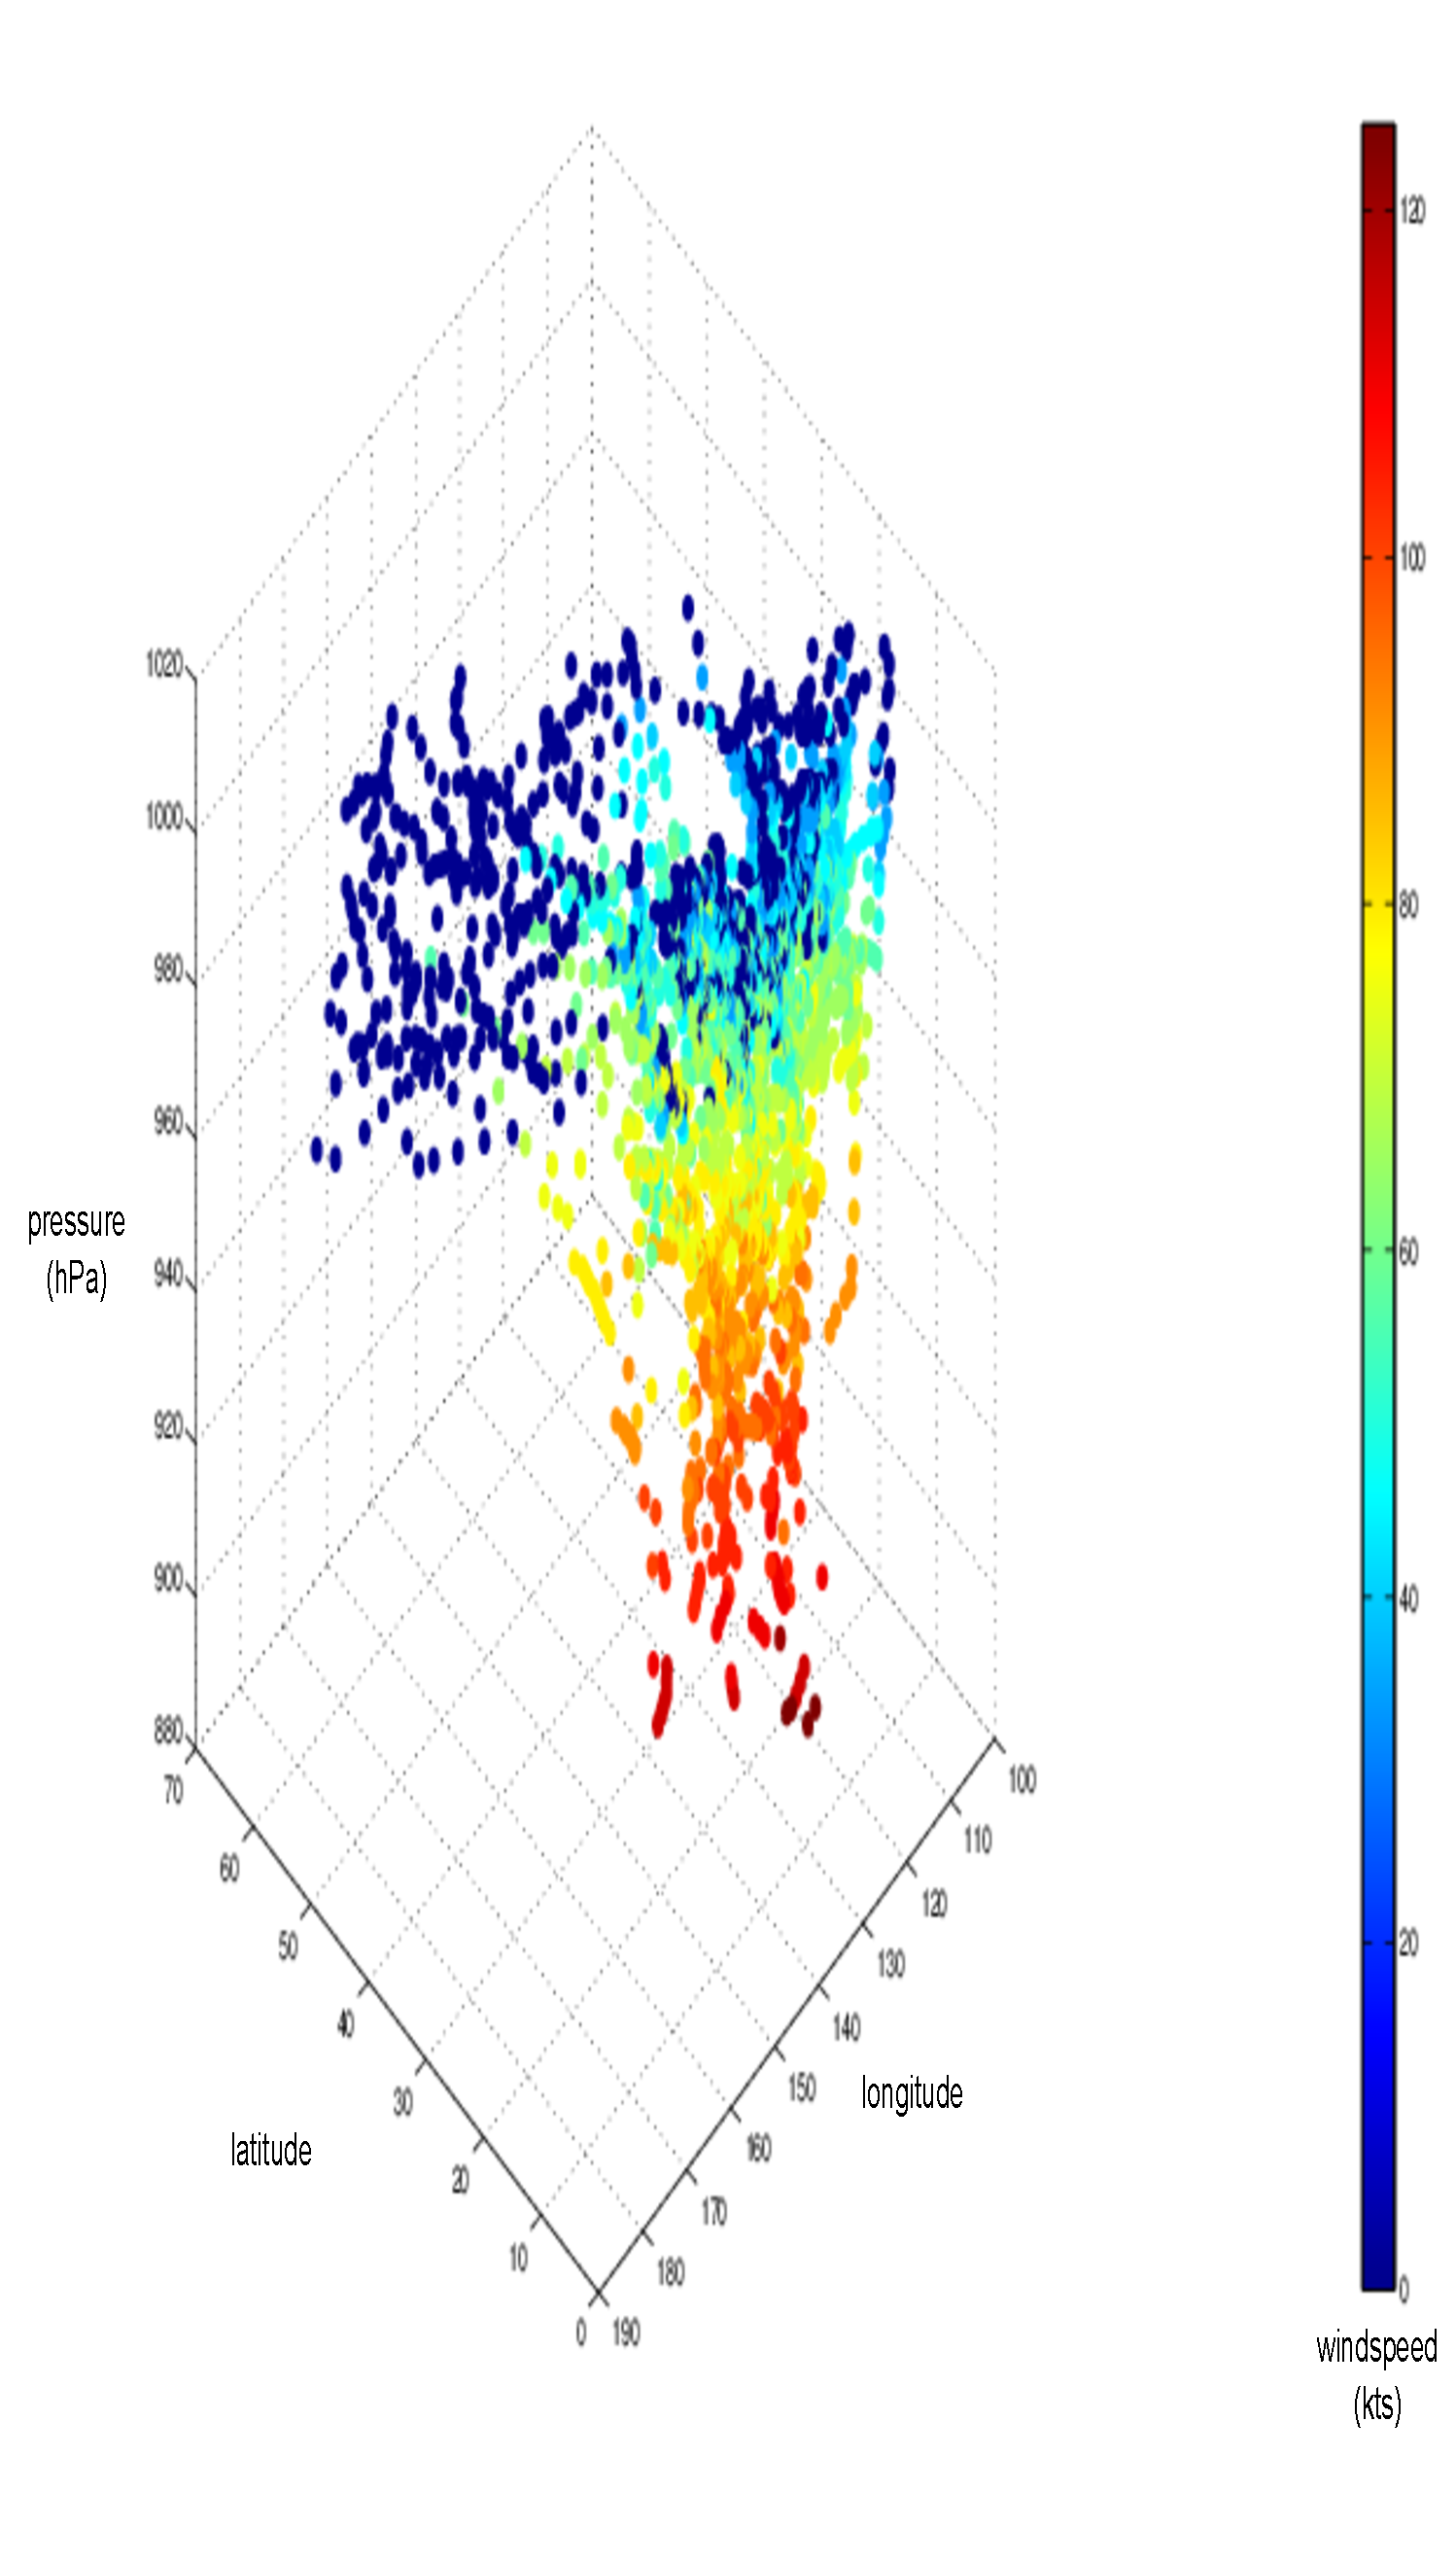
\includegraphics[width=5.75in,height=5in]{violentfig1a.eps}
\caption{Best tracks of JMA Grade 5 typhoons (2009-2012) with points colored by recorded best track wind speeds (in knots). Genesis points are shown in dark blue (at the right half) and violent points in red. Track points separated by 6 hour intervals form a ``funnel" which narrows with increased wind speeds and decreased pressure.}
\label{fig1a}
\end{figure}

\newpage

 \begin{figure}[h]
 \centering
\includegraphics[width=6in,height=4in]{violentfig1.eps}
\caption{Violent points of  2009-2012 typhoons (shown in bold) are confined to a rectangle [122$^{\textup{o}}$E,145$^{\textup{o}}$E] x [12.5$^{\textup{o}}$N,20$^{\textup{o}}$N].}
\label{fig1}
\vspace{2in}
\end{figure}



\newpage
 \begin{figure}[!htpb]
 \centering
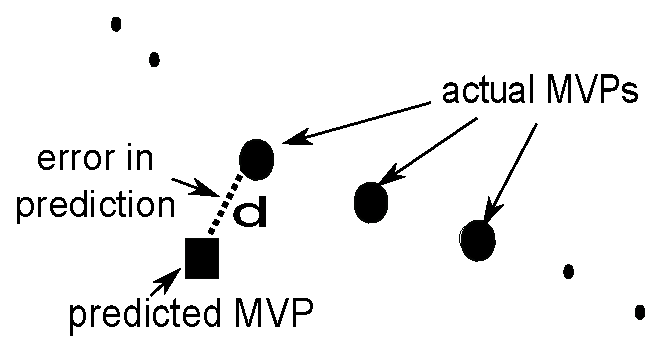
\includegraphics[width=3in,height=1.75in]{violentfig2.eps}
\caption{Distance used to compute the error in a predicted most violent point (MVP).}
\label{fig2}
\vspace{5in}
\end{figure}

\newpage

 \begin{figure}[!htpb]
 \centering
\includegraphics[width=5.5in,height=3.75in]{violentfig3.eps}
\caption{Genesis points (GPs) and most violent points (MVPs) of 2009-2012 violent typhoons. GP Window:[134.7$^o$E x 160.4$^o$E]x [6.7$^o$N,14.3$^o$N]; MVP Window: [123.3$^o$E x 145.0$^o$E]x [13.6$^o$N,19.2$^o$N]}
\vspace{5in}
\label{fig3}
\end{figure}

\newpage


 \begin{figure}[!htpb]
 \centering
\includegraphics[width=5.5in,height=3.75in]{violentfig4.eps}
\caption{Monte Carlo simulation of the 2013 average predicted MVP position errors (n=1000)}
\vspace{5in}
\label{fig3}
\end{figure}



\newpage

\begin{table}[!htpb]
\centering
\begin{tabular}{ll}
\multicolumn{2}{c}{{\bf \large List of Tables}}\\
& \\
1 & Genesis Points and Violent Points of 2009-2012 Violent Typhoons.....27 \\
2 & Default Model Regression Coefficients................................................28\\
3 & Default Model Error in Predicted Most Violent Points (MVPs).............29\\
4 & Error in Predicted MVPs Using a Geographic Distance Filter..............30\\
5 &  General Algorithm to Find the  GP/MVP Model's EGP Error................31\\
6 &  EGP Error Comparisons......................................................................32\\

\end{tabular}
\end{table}


\newpage
\begin{table}[h]
\tiny
\centering
   \begin{tabular}{|l|c|l|c|c|c|c|}
 \multicolumn{7}{c}{{\small Table 1. Genesis Points and Violent Points of 2009-2012 Violent Typhoons}} \\\hline
 typhoon&data type&time(hrs) & lat & lon & pressure (hPa)&max wind speed (knots)\\\hline
1. Choi-wan &genesis point&  0	&14.3	&153.5	& 1008	& -	\\
(2009)&most violent point &84&	17.9&	145.0&	915&	105	\\
&most violent point&90&	18.2&	144.2&	915&	105	\\
&most violent point&96&		18.6&	143.4&	915&	105	\\
&most violent point&102&		19.0&	142.6&	915&	105	\\
&most violent point&108&		19.2&	141.9&	915&	105	\\
&most violent point&114&19.6&141.4&915&105\\\hline
2. Melor & genesis point &0	    &9.6	&160.4	&1002&	-\\	
(2009) &violent point&114	&16.6&	142.3&	920&    105	\\	
&most violent point&120	&17.0&	140.9&	910&	110	\\	
&most violent point&126	&17.5&	139.4&	910&	110	\\	
&most violent point&132	&17.9&	137.7&	910&	110	\\	
&violent point&138	&18.5&	136.3&	915&	105	\\
&violent point&144	&19.2&	134.8&	915&	105	\\\hline
3. Nida&genesis point &0&	6.7	&148.3	&1002&	-	\\
(2009) &violent point&90	&12.6	&142.2	&925&	105	\\
&most violent point&96	&13.6	&141.4	&905&	115	\\
&most violent point&102&	14.5&	140.7&	905&	115	\\
&violent point&108&	15.2&	140.0&	905&	110	\\
&violent point&114&	15.8&	139.7&	915	&105	\\
&violent point&120&	16.3&	139.3&	915	&105	\\   \hline
4. Megi&genesis point &0	&11.9	&141.4	&1006&	-	\\
(2010) &violent point&96	&18.7	&127.5	&915	&105	\\
&violent point&102&	18.5	&126.2&	905	&110	\\
&violent point&108&	18.1	&125.1	&895&	120	\\
&most violent point&114&	17.6	&124.2	&885&	125	\\
&most violent point&120&	17.5	&123.3	&885&	125	\\
&violent point&126&	17.1	&121.9	&910&	105	\\\hline
5. Songda&genesis point & 0&	83	&1416&	1006&	-	\\
(2011) &most violent point&156&	15.6	&1258	&920&	105	\\
&most violent point&162&	16.2	&125.1	&920&	105	\\
&most violent point&168&	17.2	&124.5	&920&	105	\\
&most violent point & 174	& 18.1&	123.9	&920&	105\\\hline
6. Sanba&genesis point &0&	8.7&	134.7&	1008&	-	\\
(2012) &violent point&84	&16.3&	129.6&	910	&105	\\
&most violent point&90	&17.2&	129.7&	900	&110	\\
&most violent point&96	&18.1&	129.7&	900	&110\\
&most violent point & 102 &	19.1	&129.8	&900&110\\\hline	
7. Jelawat&genesis point &0	&13.7&	134.8&	1010&	-	\\
(2012) &violent point&108&	14.6	&128.1&	910	&105	\\
&most violent point&114&	15.2	&127.9&	905	&110	\\
&most violent point&120&	15.7&	127.8&	905&	110\\	
&most violent point&126&	16.4&	127.5&	905&	110	\\
&most violent point&132&	16.8&	127.1&	905&	110	\\
&most violent point&138&	17.1&	126.8&	905&	110	\\
&most violent point&144&	17.4&	126.5&	905&	110	\\
&most violent point&150&	18.0&	126.1&	905&	110	\\
&most violent point&156&	18.4&	125.9&	905&	110	\\
&violent point&162&	19.1&	125.4&	915&	105	\\\hline
\end{tabular}
\end{table}


\newpage

\begin{table}[!htpb]
\begin{center}
\begin{tabular}{|c||c|c|c|c|}
 \multicolumn{5}{c}{{\normalsize Table 2. Default Model Regression Coefficients}}\\
 \multicolumn{5}{c}{A) Based on 2009-2012 GP/MVP Data} \\
\hline
\multicolumn{1}{|c||}{} & \multicolumn{4}{c|}{PREDICTORS} \\ \hline
\multicolumn{1}{|c||}{FORECAST} & constant & lat & lon & pressure \\ \hline
\multicolumn{1}{|c||}{Time} & 3142.314 & 0.406 & -1.367 & -2.808 \\ \hline
\multicolumn{1}{|c||}{Latitude} & -708.140 &  -0.254 & 0.167 &  0.699 \\ \hline
\multicolumn{1}{|c||}{Longitude} & -1827.084 &  -0.799 &  1.033 & 1.807 \\ \hline
\multicolumn{1}{|c||}{Pressure} &   -6003.952 & -4.693 &  1.649 & 6.681 \\ \hline
\multicolumn{1}{|c||}{Wind Speed} & 5339.129 &  3.236 &  -1.076 & -5.076 \\ \hline\hline
 \multicolumn{5}{c}{B) Based on 2010-2013 GP/MVP Data} \\\hline
 \multicolumn{1}{|c||}{FORECAST} & constant & lat & lon & pressure \\ \hline
\multicolumn{1}{|c||}{Time} & -2247.013 & -4.091 & -0.988 & 2.534 \\ \hline
\multicolumn{1}{|c||}{Latitude} & -246.923 & 0.275 & 0.053 & 0.252 \\ \hline
\multicolumn{1}{|c||}{Longitude} & -1745.465 & 0.667 & 0.879 & 1.73 \\ \hline
\multicolumn{1}{|c||}{Pressure} & 907.724 & 0.927 & 0.125 & -0.028 \\ \hline
\multicolumn{1}{|c||}{Wind Speed} & 1053.239 & -0.288 & 0.121 & -0.949 \\ \hline
\end{tabular}
\end{center}
\vspace{3in}
\end{table}

\newpage

\begin{table}[!htpb]
\tiny
\begin{center}
\begin{tabular}{c||c|c|c|c|c||c|c|c|c|c||c|c|c||c|c|}
 \multicolumn{16}{c}{{\small Table 3. Default Model Error in Predicted MVPs}} \\
  \multicolumn{16}{c}{{}} \\
  \multicolumn{16}{c}{{\small A) 2013}}\\\hline
 \multicolumn{6}{|c||}{Predicted MVP} & \multicolumn{5}{|c||}{Closest Actual MVP}& \multicolumn{3}{|c||}{Error} & \multicolumn{2}{|c|}{JMA}\\
\cline{1-16}
\multicolumn{1}{|m{.2in}||}{Storm Name} & \multicolumn{1}{|m{.3in}|}{Time (hrs)} &\multicolumn{1}{|m{.2in}|}{Lat $^o$N}& \multicolumn{1}{|m{.2in}|}{Lon $^o$E}  & \multicolumn{1}{|m{.3in}|}{Pres (hPa)} &  \multicolumn{1}{|m{.2in}||}{Wind Speed (knots)} & Time & Lat & Long & Pres & WS & Position & WS & Time &   EO &EP  \\\hline
\multicolumn{1}{|c||}{Utor} & 130.3 & 16.6 & 126.1 & 898.9 & 114.9 & 72 & 15.5 & 123.5 & 925 & 105 & 300 & 9.9 & 58.3 &286 & 572 \\
\multicolumn{1}{|c||}{Usagi} & 144.3 & 13.1 & 113.6 & 853.6 & 146.9 & 108 & 20.1 & 123.8 & 910 & 110 & 1340.4 & 36.9 & 36.3 & 235  & 1236.8  \\
\multicolumn{1}{|c||}{Francisco} & 114.1 & 18.2 & 137.4 & 911.2 & 107.2 & 102 & 17.4 & 138.3 & 920 & 105 & 51.8 & 2.2 & 12.1 & 256  & 624.4  \\
\multicolumn{1}{|c||}{Lekima} & 93.9 & 21.6 & 155.0 & 954.6 & 78.1 & 96 & 18.6 & 152.2 & 905 & 115 & 439 & 36.9 & 2.1 & 395   & 963.4  \\
\multicolumn{1}{|c||}{Haiyan} & 110.8 & 18.8 & 145.2 & 935.7 & 92.7 &  102 & 10.2 & 129.1 & 895 & 125 & 1973.8 & 32.3 & 8.8 & 401  & 853.2  \\\hline\hline
\multicolumn{11}{|r||}{Average}&\multicolumn{1}{|m{.2in}|}{\vspace{.1in} 821.1 \hspace{.5in} ({\bf p}=.155)} &23.64&23.52&314.6&850.0\\\hline
  \multicolumn{16}{c}{}\\
\multicolumn{16}{c}{{\small B) 2014}} \\\hline
\multicolumn{6}{|c||}{Predicted MVP} & \multicolumn{5}{|c||}{Closest Actual MVP}& \multicolumn{3}{|c|}{Error} & \multicolumn{2}{||c|}{JMA}\\\hline
\multicolumn{1}{|m{.2in}||}{Storm Name} & Time & Lat & Lon & Pres & WS & Time & Lat & Lon & Pres & WS & Position & WS & Time & EO & EP \\
\hline
\multicolumn{1}{|c||}{Halong} & 105.6 & 17.2 & 136.1 & 908.8 & 113.7 & 138 & 14.9 & 135.1 & 920 & 105 & 282 & 8.7 & 32.4 & 528 & 1123.4\\
\hline
\multicolumn{1}{|c||}{Genevieve} & \multicolumn{15}{|l|}{(genesis point not available)}\\
\hline
\multicolumn{1}{|c||}{Vongfong} & 111.7 & 16.7 & 142.5 & 906.4 & 116.1 & 126 & 17.7 & 133.2 & 900 & 115 & 992 & 1.1 & 14.2 & 329  & 1827.8\\
\hline
\multicolumn{1}{|c||}{Nuri} & 105.9 & 16.5 & 123.9 & 908.7 & 113.9 & 90 & 17.8 & 132.4 & 910 & 110 & 910 & 3.9 & 15.9 & 521  & 1371.1\\
\hline
\multicolumn{1}{|c||}{Hagupit} & 137 & 15.1 & 134 & 901.2 & 116.7 & 96 & 11 & 131.3 & 905 & 115 & 539 & 1.7 & 41 & 161 & 1006.3\\\hline\hline
\multicolumn{11}{|r||}{Average}&\multicolumn{1}{|m{.2in}|}{\vspace{.1in} 681.0 \hspace{.5in} ({\bf p}=.57)} &3.85&25.9&384.75&1332.15\\\hline
\end{tabular}
\end{center}
\end{table}


\newpage

\begin{table}[!htpb]
\tiny
\begin{center}
\begin{tabular}{c||c|c|c|c|c||c|c|c|c|c||c|c|c||c|c|}
 \multicolumn{16}{c}{{\small Table 4. Error in Predicted MVPs Using a Geographic Distance Filter}} \\
 \multicolumn{16}{c}{GP/MVP data for 3 Closest Storms Used in Prediction.} \\
  \multicolumn{16}{c}{{}} \\
  \multicolumn{16}{c}{{\small A) 2013}}\\\hline
 \multicolumn{6}{|c||}{Predicted MVP} & \multicolumn{5}{|c||}{Closest Actual MVP}& \multicolumn{3}{|c||}{Error} & \multicolumn{2}{|c|}{JMA}\\
\cline{1-16}
\multicolumn{1}{|m{.15in}||}{Storm Name} & \multicolumn{1}{|m{.3in}|}{Time (hrs)} &\multicolumn{1}{|m{.15in}|}{Lat $^o$N}& \multicolumn{1}{|m{.2in}|}{Lon $^o$E}  & \multicolumn{1}{|m{.3in}|}{Pres (hPa)} &  \multicolumn{1}{|m{.2in}||}{Wind Speed (knots)} & Time & Lat & Lon & Pres & WS & Position & WS & Time &   EO &EP  \\\hline
\multicolumn{1}{|c||}{Utor} & 121.4 & 17.3 & 126.59 & 897.8 & 114.2 & 72 & 15.5 & 123.5 & 925 & 105 & 387.2 & 9.2 & 49.4 &286 & 572 \\
\multicolumn{1}{|c||}{Usagi} & 164.1 & 15.8 & 125.4 & 908.4 & 104.8 & 90 & 18.7 & 126.4 & 910 & 110 & 343.9 & 5.2 & 74.1 & 235  & 1236.8  \\
\multicolumn{1}{|c||}{Francisco} & 106.5 & 18.5 & 135.3 & 903.7 & 112.7 & 108 & 17.8 & 137.7 & 920 & 105 & 268.6 & 7.7 & 1.5 & 256  & 624.4  \\
\multicolumn{1}{|c||}{Lekima} & 130 & 17.6 & 139.9 & 915.6 & 111.1 & 126 & 21.4 & 146.5 & 905 & 115 & 817.7 & 3.9 & 4 & 395   & 963.4  \\
\multicolumn{1}{|c||}{Haiyan} & 123.1 & 15&139.3 & 909.1 & 115.7 &  102 & 10.2 & 129.1 & 895 & 125 & 1225.54 & 9.3 & 21.1 & 401  & 853.2  \\\hline\hline
\multicolumn{11}{|r||}{Average}&\multicolumn{1}{|m{.2in}|}{\vspace{.1in} 608.6 \hspace{.5in} ({\bf p}=.008)} &7.06&30.02&314.6&850.0\\\hline
  \multicolumn{16}{c}{}\\
\multicolumn{16}{c}{{\small B) 2014}} \\\hline
\multicolumn{6}{|c||}{Predicted MVP} & \multicolumn{5}{|c||}{Closest Actual MVP}& \multicolumn{3}{|c||}{Error} & \multicolumn{2}{|c|}{JMA}\\\hline
\multicolumn{1}{|m{.15in}||}{Storm Name} & Time & Lat & Lon & Pres & WS & Time & Lat & Lon & Pres & WS & Position & WS & Time & EO & EP \\
\hline
\multicolumn{1}{|c||}{Halong} & 95.7 & 14.7 & 136.3 & 912.8 & 110.4 & 138 & 14.9 & 135.1 & 920 & 105 & 133.2 & 5.4 & 42.3 & 528 & 1123.4\\
\hline
\multicolumn{1}{|c||}{Genevieve} & \multicolumn{15}{|l|}{(genesis point not available)}\\
\hline
\multicolumn{1}{|c||}{Vongfong} & 111 & 16.5 & 142.1 & 898.6 & 120.3 & 126 & 17.7 & 133.2 & 900 & 115 & 958.7 & 5.3 & 15 & 329  & 1827.8\\
\hline
\multicolumn{1}{|c||}{Nuri} & 105.6 & 17.6 & 123.3 & 877.6 & 128 & 90 & 17.8 & 132.4 & 910 & 110 & 967.1 & 18 & 15.6 & 521  & 1371.1\\
\hline
\multicolumn{1}{|c||}{Hagupit} & 103.6 & 3.9 & 114.2 & 889.9 & 134.4 & 102 & 11.4 & 130.4 & 905 & 115 & 1969.9 & 19.4& 1.6 & 161 & 1006.3\\\hline\hline
\multicolumn{11}{|r||}{Average}&\multicolumn{1}{|m{.2in}|}{\vspace{.1in} 1007.2 \hspace{.5in} ({\bf p}=.886)}  &12.03 &18.63&384.75&1332.15\\\hline
\end{tabular}
\end{center}
\vspace{3in}
\end{table}







\newpage

\begin{table}[!htpb]
\scriptsize
\begin{center}
\begin{tabular}{|l|}
\multicolumn{1}{c}{{\small Table 5. General Algorithm to Find the  GP/MVP Model's EGP Error}}\\
\multicolumn{1}{c}{}\\\hline
 \multicolumn{1}{|m{5in}|}{ 1. {\bf READ} (GP(X),MVP(X)),  the genesis point and most violent point(s) of  storm X, for all X in 2009-2012.}\\
  2. {\bf FOR} each violent typhoon S in 2013\\
     \hspace{.25in} begin\\
\hspace{.5in} 2a. {\bf READ} GP(S), storm S's genesis point lat, lon and pressure.\\
 \hspace{.5in} 2b. {\bf  INCLUDE}  (GP(X),MVP(X)) in the data used in regression (DUIR) if distance(GP(X),GP(S)) $< r$.\\
  \hspace{.5in} 2c. {\bf  COMPUTE} the regression coefficients for the DUIR constructed in step 2b.\\
\hspace{.5in}  2d. {\bf  COMPUTE} MVP$^*$(S),  a predicted most violent point of S, using the coefficients in step 2c.\\
   \multicolumn{1}{|m{5in}|}{\hspace{.5in} 2e. {\bf COMPUTE} ERROR(S)= the (minimum) geographic distance between the predicted}\\
    \multicolumn{1}{|m{5in}|}{\hspace{.75in}  MVP$^*$(S) and an actual MVP(S).}\\
    \hspace{.25in} end\\
\multicolumn{1}{|m{5in}|}{3. {\bf COMPUTE} EGP, the average of ERROR(S) over all S in 2013.}\\\hline
\end{tabular}
\end{center}
\vspace{5in}
\end{table}






\newpage


\begin{table}[!htpb]
\begin{center}
\begin{tabular}{|c||c|c|c|}
\multicolumn{4}{c}{{\small Table 6. EGP Error (km) Comparisons }}\\ \hline
Method & 2013$^{\scriptsize 1}$ & 2014$^{\scriptsize 1}$ & 2015$^{\scriptsize 2}$\\\hline\hline
Default & 821.1 ({\bf p}=.16) & 681.3 ({\bf p}=.57) & 583.0 ({\bf p}$<$.001)\\\hline\hline
Taxicab metric ($r$=3) & 537.8 ({\bf p}$<$.01) & 609.7 ({\bf p}=.47) & 3096.8 ({\bf p}$>$.999)\\\hline
Taxicab metric ($r$=4) & 851.4 ({\bf p}=.21) & 1094.6 ({\bf p}=.92) & 779.6 ({\bf p}=.052)\\\hline
Taxicab metric ($r$=5) & 1065.2 ({\bf p}=.64) & 634.0 ({\bf p}=.51) & 672.4 ({\bf p}=.005)\\\hline
Euclidean norm ($r$=3) & 760.7 ({\bf p}=.08) & 872.4 ({\bf p}=.79) & 611.4 ({\bf p}=.001)\\\hline
Euclidean norm ($r$=4) & 1070.0 ({\bf p}=.66) & 790.8 ({\bf p}=.71) & 583.0 ({\bf p}$<$.001)\\\hline
\end{tabular}
\end{center}
\hspace{3in} {\scriptsize $^1$1000 randomized trials; $^2$10,000 randomized trials.}
\end{table}



\end{document}

